\section{Laboratorio No 06 – Cuestionario} 

\begin{enumerate}[1.]
	\item ¿Qué sucede al ejecutar los siguientes comandos?
	\begin{center}
	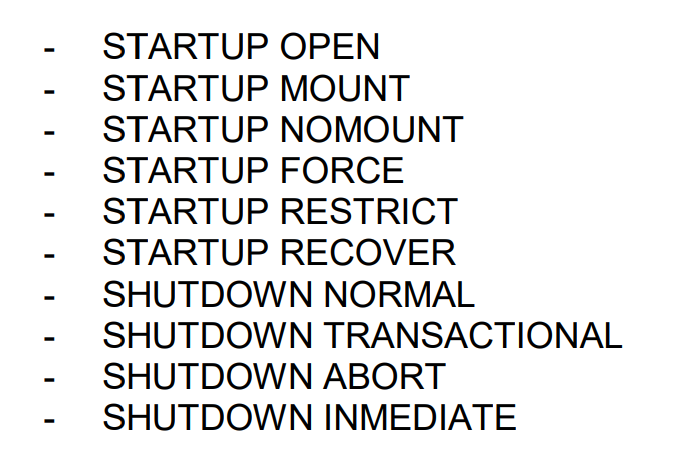
\includegraphics[width=8cm]{./Imagenes/actividad_5_1_lab_06}
	\end{center}	

	\item . En el script lab\_02\_01.sql, se establecen privilegios de sistema, enliste los privilegios de sistema (DDL) utilizados y describa cada uno de ellos.
	\\\\- create table 
	\\- insert into
	\\- exec
	\\- begin tran
	\\- save tran
	\\- delete
	\\- select
	\\- rollback tran
	\\- alter proc
	\\- declare
	\\-  create sequence
	\\- drop sequence
	\\- create index
	\\- creatw synonym
	
	\item Enliste y describa los tipos de TableSpace que existen en Oracle.
	\\\\ existen dos tipos de tablespace :
	\\- TableSpace System	: se crea automaticamente al hacer la instalacion de oracle o al crear una BD.
	\\- TableSpace Temporales	: es aquel en el que solamente puede haber objetos temporales
	\\\\- de tipo deshacer cambios	: se utilizan para gestionar poder deshacer las transacciones incompletas.
	\\- con tamaño de bloque variable
	\\- de tipo BigFile	
	

\end{enumerate} 
